%!TEX root = ../../main.tex

\chapter{Introduction}

The project is about predicting the outcome of soccer games and training a neural network. For the training the database from Kaggle in source \cite{kggl:2019} has been used. 


\section{Motivation}
 Machine Learning and Neural Networks is a main topic in the software development field. Many companies start to try analyze different kind of data with this approach. Because of this reason as master students in information systems it is very interesting to gather knowledge about machine learning and neural networks. For this matter a prediction of soccer matches is a very nice procedure to do. For this topic there is not many additional knowledge to gather, what you need for analyzing the data and prepare them for prediction. Additionally there is a free database with data of matches for a couple of years. In the beginning the knowledge about machine learning is very low and the goal is to improve the handling of python in combination with machine learning techniques. This includes pre-processing data with Pandas, normalizing data sets and extracting the right features, as well as developing adequate models for the machine-learning algorithm. Additionally to the gaining of knowledge we like to create an algorithm, which predicts the outcome of soccer games with a decent accuracy.
\section{Goals}
The main goals of this project can be divided into 2 parts:
\begin{itemize}
	\item \textbf{Gaining knowledge}
		\begin{itemize}
			\item Improve skills in python\newline
			For the the project and for future work with neural networks it is necessary to become familiar with python. There are many things, which are different in python than in other programming languages. All these things have to be discovered and it is necessary to learn how to deal with the python syntax. Additionally its important to gain knowledge about some library, which you can use with python and make it easier to solve some problems.
			\item Gaining knowledge about data pre-processing\newline 
			It is very important to edit the data in a way, that it is ready for a neural network. Algorithms can for example not deal with strings, only with numbers. For this matter, before there has to be some knowledge gained, that the data can be processed in a proper way.
			\item Gaining knowledge about neural networks\newline
			Neural networks is one of the most famous topics in the technical world these times. So as master students in computer science it is urgent to gain some knowledge about neural networks and machine learning. For the project it is necessary too to understand the overall technology of the whole topic. 
		\end{itemize}
	\item \textbf{Outcome of the project}
		\begin{itemize}
			\item Finding the right features \newline
			As a first step it should be done a feature selection. For this the database has to be analyzed and there should be choose some first features by gut feeling. This features has to be checked, if they are independent of each other. During the project it should be always reconsidered, if it make sense to add some more features and checked whether it improves the accuracy. 
			\item Normalizing the features in a proper way \newline
			The features have to be normalized before using them for a prediction model. For this procedure it is necessary to find algorithms or write some. The normalization of the data is a major step in the project development.
			\item Finding a good model for the prediction 
			There are different libraries available for machine learning. The recommended library is Tensorflow in combination with Keras. Additional there has to be research for other libraries and approaches. The different models are compared and in the end the best model will be choose. 
			\item Getting a decent accuracy with the prediction \newline
			The accuracy should be higher than 50\% in the end. With more than 50\% you would theoretically always earning money, if you would bet everything, which the model is predicting. The main goal is to improve the accuracy during the whole project. 
		\end{itemize}
\end{itemize}
\section{Procedure}

For the procedure process we decided to proceed in order to the CRISP-DM model. In image \ref{CRISImage} you can see the different stages in order to CRISP-DM.

\begin{figure}[h]
\centering
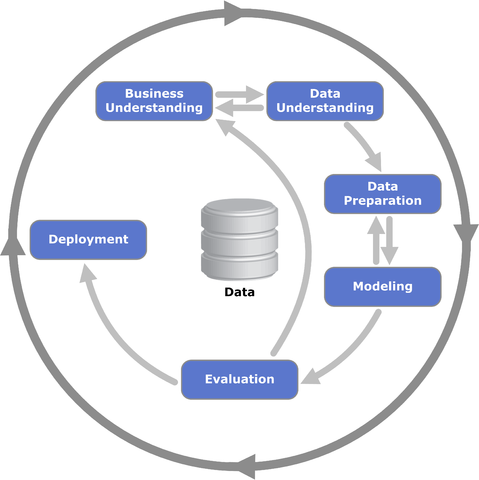
\includegraphics[width=0.5\textwidth]{images/CRISP-DM_Process_Diagram1.png}
\caption{The six stages of CRISP-DM \cite{CRISPDig:2012}}
\label{CRISImage}
\end{figure}

\begin{itemize}
\item Business Understanding \newline
As first step we have to set the goals of the project which are already described in the chapter before. It is necessary to clear what exactly is the required outcome. For this matter in this project we use SCRUM to organize our project. We meet once per week to discuss the achievements from each single person. All 3-4 weeks there is a sprint meeting where we discuss the group achievements and if the project still leads to the right way. In the initial sprint meeting the common parameters of the project are set. 
\item Data Understanding \newline
Before we can start to create a model or select features we have to understand the Dataset. For this matter it is necessary to understand the structure of the set including the different columns and what they indicate. Additional it is important how many data the set includes and which types of value. It is important to learn also something about soccer and what are important facts about a game. 
\item Data Preparation \newline
 Before it is possible to use the Dataset in a neuronal network it is necessary to prepare the data. For this matter as first step there has to be a feature selection. So one has to decide which columns are important for the later prediction. After we dropped the unnecessary columns it is important to prepare the resulting dataset. The records which have empty attributes have to be deleted or filled with specific values. Additionally the data has to be sorted and aggregated. At the end it has to be split into test and training data. 
 \item Modeling \newline
 The resulting dataset from the step before should be ready to be used for different models. In this step we will prepare different models to find a decent one. Additionally it is necessary to define a measurable goal how good the model can get.   
\item Evaluation \newline
In the end of this semester we will make a evaluation of the accomplished goals and if it is possible to increase the accuracy in the following semester.  
\end{itemize}

The steps `Data Preperation' and `Modeling' will repeat as long as the resulting accuracy is not getting any better or we are satisfied with the resulting one. For all the steps it is necessary to do a lot of research to find the right techniques to do the tasks in a proper way. 